\section{Performance Evaluation}

%The evaluation of \sys can be divided into two parts. We develop a virtual network environment with Mininet which is able to build complex network topology and run real data transmission by virtualizing multiple kernels. The bandwidth is limited to simulate the real WAN environment and we program the virtual kernels to train and communicate according to the protocols of federated averaging algorithm and \sys. Note that in the network simulation, the kernel performs pseudo-training which only consumes time but trains nothing. On the other hand, we perform the training process on a single machine with 4x NVIDIA GTX 1080 Ti graphic cards. The training process is logically identical with the real distributed systems only but it executes the training of each node sequentially. Some details are as follows:

\subsection{Setup}

We conduct simulation experiments to evaluate our design. The evaluation can be divided into two parts. First, the stateful and synchronous nature of \sys allows us to simulate the training process sequentially, while logically, the training result is the same as the parallelized way. The training traces of each worker are then recorded, which contains the validation accuracies, training iterations, and corresponding synchronization partners. Second, we simulate the network topology and feed it with the training traces to estimate the training time. The specific settings are listed as follows:

$\triangleright$ \textit{Training settings.} We train a CNN model on CIFAR-10 dataset to evaluate the training ability of \sys. The dataset consists of  50,000 images for training and 10,000 for validation. The training data are randomly distributed among the workers without overlapping, and the validation data are shared among every worker. The CNN model is adopted from \cite{McMahan2017FL}, which is considered to be suitable for CIFAR-10 dataset. 

The models are trained on each worker using SGD algorithm with the same hyper-parameters, that a learning rate of 0.1 and a batch size of 128. The synchronization interval is set to 40, which means every worker perform SGD updates on the local model for 40 times before it communicates with others.

$\triangleright$ \textit{Network settings.} We simulate a fully connected network topology among the workers. The maximum bandwidth limit of each worker is set to be 100Mbps. Moreover, to simulate the bottleneck of WAN, we set 10Mbps as the available bandwidth between two workers.

$\triangleright$ \textit{Comparison settings.} We compare \sys and (1) traditional federated learning system with a \emph{centralized} parameter server and (2) naive \emph{gossip} approach without segmentation. To make them comparable, they are all simulated within the same network topology, and for the centralized system, we randomly choose one worker to play the role of parameter server.

The communication behavior of \sys is controlled by two parameters: \emph{model segments} as $S$ and \emph{model replica} as $R$. In our following experiments, we set $S=10$ and $R=2$ by default, that is in the synchronization phase, the model is partitioned into ten segments, and for each segment, the worker requests two replicas from other workers. The gossip approach is the special case of \sys when $S=1$, and it shares the same value of $R$ with \sys.


$\triangleright$ \textit{Performance Metrics.} The learning performance is measured by the convergence speed. We record the top-1 validation accuracies of the aggregated models at each round and then align the accuracies to the corresponding times. The time is acquired from our network simulator where the local update time is referenced from the real machine time of training with a GTX 1080 Ti graphics card, and the communication time is calculated according to the bandwidth limitations.


\subsection{Experiment Result}

We first evaluate the convergence speed and scalability of \sys in comparison to the other approaches, then we explore the advantages and disadvantages of the design of model segments and replicas and how they affect the training performance.

\subsubsection{Convergence Speed}

We present the whole training process over time, as illustrated in Fig.\ref{Fig: time_acc_30}, \sys exhibits an apparent speedup in the convergence without affecting the final validation accuracy. We also explore the scalability of these three methods by comparing the training time needed to reach a predefined accuracy goal with varying number of workers among 20, 30, and 40. According to Fig.\ref{Fig: time_acc_30}, the model reaches convergence around 82\% validation accuracy. Since the aim is not achieving the best accuracy and practically speaking, it is not worthy of spending too much time for only 1\% or 2\% accuracy gain. Thus we set 80\% as the accuracy goal. 

As illustrated in Fig.\ref{Fig: scale_time}, \sys requires the least training time to reach the given accuracy within all three cases and compared with the centralized system, the speedup of \sys increases from $2.25\times$ to $3.01\times$ with the expansion of scale. This phenomenon indicates that the decentralized federated learning is more scalable than the centralized way. Additionally, both as the decentralized approaches, \sys almost reduces the training time by half compared with the naive gossip solution.

%%%%%%%%%%%%%%%%%%%%%%%%%%%%%
\begin{figure*}[htbp]

\begin{minipage}[t]{0.32\textwidth}%%\centering
\subfigure[Convergence with 30 workers]{
\label{Fig: time_acc_30}
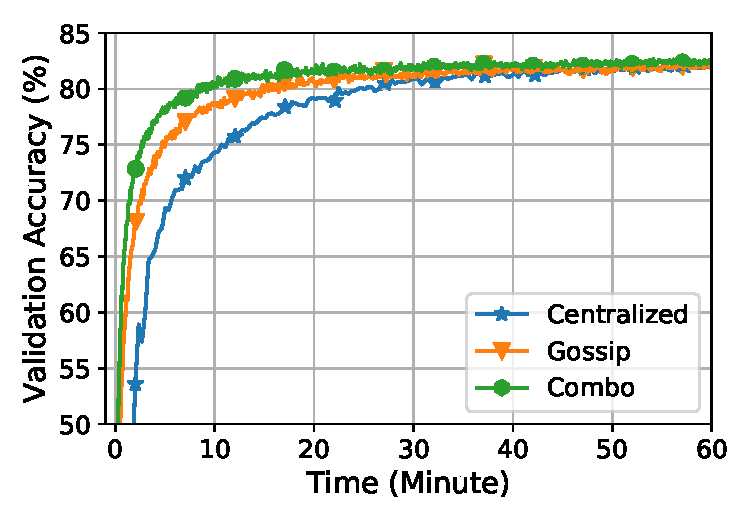
\includegraphics[width=0.9\textwidth]{pics/time_acc_30_refill.pdf}}
\\
\subfigure[Time to reach 80\% accuracy]{
\label{Fig: scale_time}
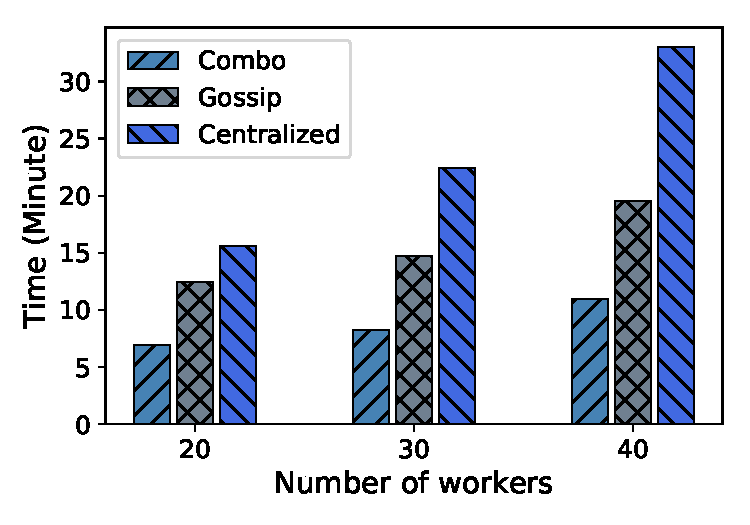
\includegraphics[width=0.9\textwidth]{pics/scale_time_refill.pdf}}

\caption{Convergence speed}
\label{Fig: acc}
\end{minipage}
\begin{minipage}[t]{0.32\linewidth}
\centering 
\subfigure[Convergence with model segments]{
\label{Fig: seg_acc}
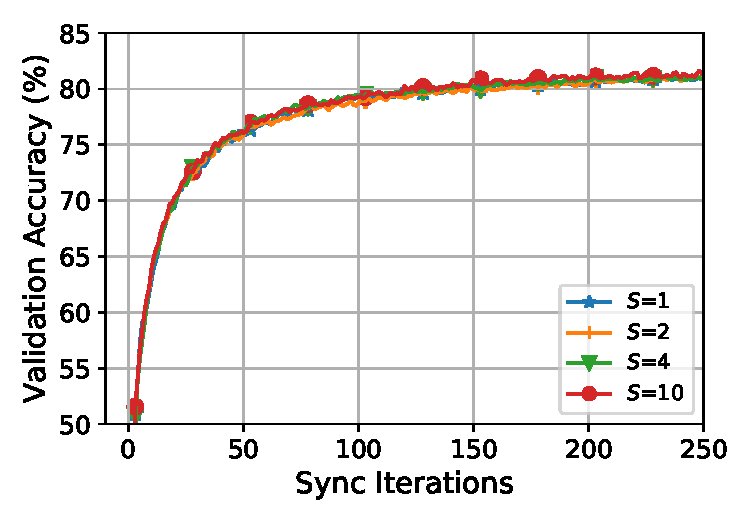
\includegraphics[width=0.9\textwidth]{pics/segment_acc_fill.pdf}}
\\
\subfigure[Sync time comparison]{
\label{Fig: seg_time}
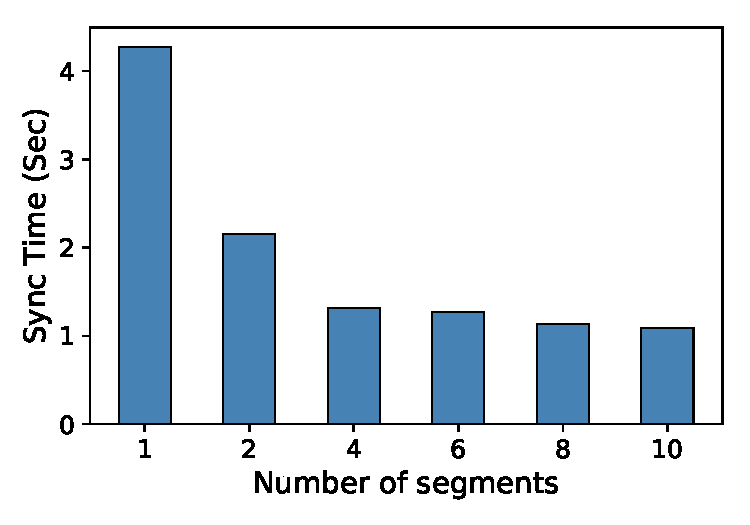
\includegraphics[width=0.9\textwidth]{pics/segment_time.pdf}}
\caption{Benefit of model segments}
\label{Fig: acc}
\end{minipage}
\begin{minipage}[t]{0.32\linewidth}
\centering 
\subfigure[Convergence with model replicas]{
\label{Fig: replica_acc}
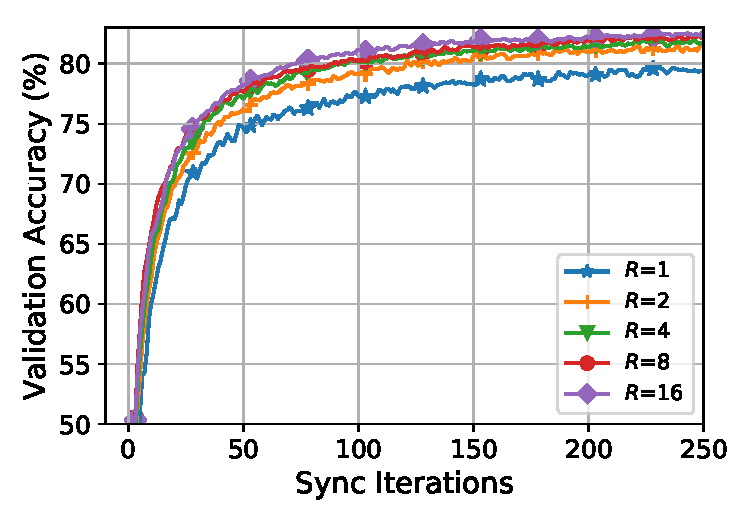
\includegraphics[width=0.9\textwidth]{pics/replica_acc_fill.pdf}}
\\
\subfigure[Time to reach 80\% accuracy]{
\label{Fig: replica_time}
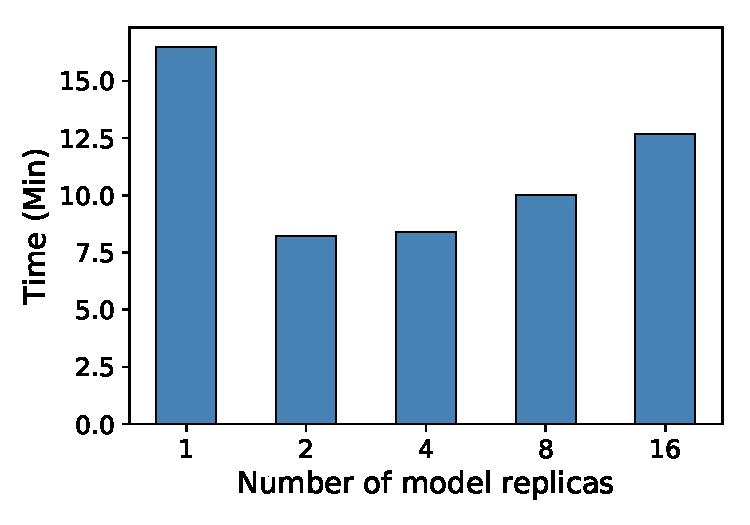
\includegraphics[width=0.9\textwidth]{pics/replica_time}}

\caption{Impact of model replicas}
\label{Fig: acc}
\end{minipage}

\end{figure*}



\subsubsection{Benefit of Model Segments}
The speedup of decentralized approaches comes from the removal of the bottleneck of the centralized server, and the advantage of \sys comes from the benefit of model segments. We train the mode with 30 workers, fix $R=2$ and vary $S$ from 1 to 10 to investigate how model segments affect the training performance.

Compared with the naive gossip solution, \sys aggregates mixed model parameters made up of multiple segments instead of the complete model. A potential concern is that the result may suffer degradation as the aggregation target is mottled and loses integrality. However, Fig.\ref{Fig: seg_acc} shows that the accuracy of the aggregated results at each synchronization iterations is not affected by the model segments at all. Partitioning the model into ten segments($S=10$) has the same convergence trend as that without partition.

While the model segments don't affect the accuracy at each iteration, the synchronization time is significantly reduced. As illustrated in Fig.\ref{Fig: seg_time}, by simply splitting the model parameters into two segments can reduce the synchronization time by half. This is because when $S=2$, the original transmission quantity is divided into two parts and fed into $2\times$ more links. When the bandwidth is not exhausted, the sending and receiving time can be reduced almost proportionally. However, when $S\geq 6$, the bandwidth is already fully exploited, increasing the number of segments will not improve the time consumption then.


\subsubsection{Impact of Model Replicas}

Next, we evaluate the impact of model replica, which controls the overall information quantity that the workers send and receive at each synchronization iterations. Similar to the previous settings, we fix $S=10$ and vary $R$ from 1 to 16.

As we discussed in the convergence analysis of \sys, the more information a worker receives, the better aggregation result it will get. When the worker receives all the model replicas from other peers, \sys becomes the All-reduce structure and achieves the same training result as the centralized approach. The analysis is validated by Fig.\ref{Fig: replica_acc} that with the increase of the number of model replicas, the accuracy of each iteration becomes better. However, the improvement is not unlimited. We can see that there is no significant gap between $R=8$ and $16$ in the convergence trend and result. This reflects the redundancy of All-reduce structure that the worker doesn't have to collect all the external models to train a high-quality model.

However, as the bandwidth of worker is fully utilized with model segments, increasing $R$ leads to the proportional growth of the transmission workload. Thus there exists a tradeoff, a larger $R$ increases the convergence rate on synchronization iterations but also the synchronization time. We compare the training time needed to reach 80\% validation accuracy with different $R$ as shown in Fig.\ref{Fig: replica_time}. Increasing $R=1$ to $2$ leads to a rapid reduction of the required training time as it drastically reduces the iterations needed to achieve target accuracy goal, which is also illustrated in Fig.\ref{Fig: replica_acc}. However, if we continue to increase $R$, the growth of the training time exceeds the reduction of the iterations and slows down the convergence speed.













